\documentclass{ctexart}

\usepackage{graphicx}
\usepackage[scale=0.8]{geometry}

\title{基于暗通道先验的单一图像去雾算法}
\author{Kaiming He, Jian Sun, and Xiaoou Tang, \emph{Fellow}, \emph{IEEE}}

\begin{document}

\maketitle

\begin{abstract}
    在这篇论文中,我们提出了一个简单但是有效的图像先验规律——暗通道先验来为单一输入图像去雾。暗通道先验来自于对户外无雾图像的统计。它基于一个关键的观察——大多数户外无雾图像存在一些在至少一个颜色通道上强度很低的像素。利用这个先验知识和雾成像模型,我们可以直接估计雾霾的厚度,并还原出高质量的去雾图像。对户外不同有雾图像的处理结果表明了我们提出的先验规律的巨大作用。同时,作为去雾过程中的副产品,我们还能得到高质量的深度图。

    \textbf{关键词:} Dehaze, defog, image restoration, depth estimation.
\end{abstract}

\section{引言}
户外场景的图像通常会因为大气中浑浊的介质(比如灰尘、水汽)而降低质量。霾、雾、烟都是大气吸收和散射而形成的现象。照相机接收到景物反射过来的光线经过了衰减。此外,得到的光线还混合有\emph{大气光}\cite{Koschmieder1924}——经大气分子反射的周围环境的光线。被降低质量的图像的对比度和颜色的保真度有所下降,如图\ref{fig:01}a所示。由于大气散射的程度和景点到照相机的距离有关,图像质量降低程度是随着空间变化的。\par

Haze removal\footnote{Haze, fog, and smoke主要在材质、尺寸、形状和大气颗粒浓度上不同。详情见\cite{NarasimhanNayar2002}。在这篇文章中我们不区分他们相似的现象,并且为了方便统一使用术语\emph{haze removal }。} (or dehazing,去雾)在消费/计算摄影业和计算机视觉领域有着广泛的需求。首先,去雾可以显著地提高景物的清晰度并且改正大气光带来的色偏。一般来说,无雾的图片看起来更加舒服。其次,大多数的计算机视觉算法,从低级别的图像分析,到高级别的目标识别,通常会假设输入图像(经过校准)是景物的场景光(scene radiance不好翻译)。视觉算法(例如特征检测、滤波、光度分析等)的实现会不可避免地受到来自有偏的和低对比度的场景光的困扰。最后,去雾可提供图像的深度信息,有助于许多视觉算法和高级的图像编辑。雾和霾可以作为有用的深度的线索来加深人们对景像的理解。一个有雾的不好的图像也可以有好的用处。\par

然而,去雾是一项有挑战性的问题,因为雾所依赖的深度信息是未知的。如果只有单个有雾图像,问题的约束就会变得过少。因此,很多使用多张图像或额外信息的去雾方法被提出。基于偏振光的方法\cite{SchechnerNarasimhanNayar2001},\cite{ShwartzNamerSchechner2006}通过不同偏振角拍摄的两张或多张图片来去除雾霾的影响。在\cite{NarasimhanNayar2000},\cite{NayarNarasimhan1999},\cite{NarasimhanNayar2003_1}里通过从同一场景在不同天气情况下的拍摄的多张照片获得更多约束。基于深度的方法\cite{KopfNeubertChenCohenCohenOrDeussenUyttendaeleLischinski2008},\cite{NarasimhanNayar2003_2}需要一些来自用户输入或已知3D模型的深度信息。\par

最近,基于单一图像的去雾取得了很大的进展\cite{Fattal2008},\cite{Tan2008}。这些方法的成功得益于更强的先验和假设。Tan\cite{Tan2008}观察到无雾图像比有雾图像具有更高的对比度,他通过扩大复原图像的局部对比度来达到去雾的效果。这样得到的结果在视觉上是很吸引人的,但可能不是实际有效的。Fattal\cite{Fattal2008}通过假设透射率和表面投影在局部是不相关的,估算景物的反照率(albedo)和介质透射率(medium transmission)。这个方法是实际有效的,可以得到令人印象深刻的结果。然而他的方法在雾霾浓度较大的时候显得无能为力,而且在假设不成立的情况下可能会失败。\par

在这篇文章,我们提出一种新的先验规律——暗通道先验,来实现单一图像去雾。暗通道先验是基于户外无雾图像的统计得出的规律。我们发现,在不包括天空的绝大部分局部区域,总会存在一些像素(我们称之为“sdark pixels”),至少在一个颜色通道上具有很低的强度值。在有雾图像中,这些颜色通道中的暗像素的强度来自于大气光。因此,这些暗像素能够直接用来评估雾的透射率。结合一个雾成像模型和soft matting插值法,我们可以修复出高质量的去雾图像并得到很好的深度图。\par

我们实现的去雾不仅是实际有效的,而且能够处理在雾浓度很大情况下的远距离物体。我们没有依靠透射率或表面投影的显著变化。结果基本没有光晕。\par

和任何其他利用强假设的算法一样,我们的方法也存在限制。当取景对象本身颜色与大气光相似(比如雪地或白墙),暗原色先验将失效。尽管我们的方法对大多数户外有雾图像有效,在一些极限情况下还是会失效。幸运的是,在那些特定场景下去雾的需求不是很强烈,因为那些时候很少看见雾。我们相信,从不同的角度来发展这一新的先验,并将他们组合起来,会进一步推动这一工作的发展。\par

\begin{figure}[tbp]
    \centering
    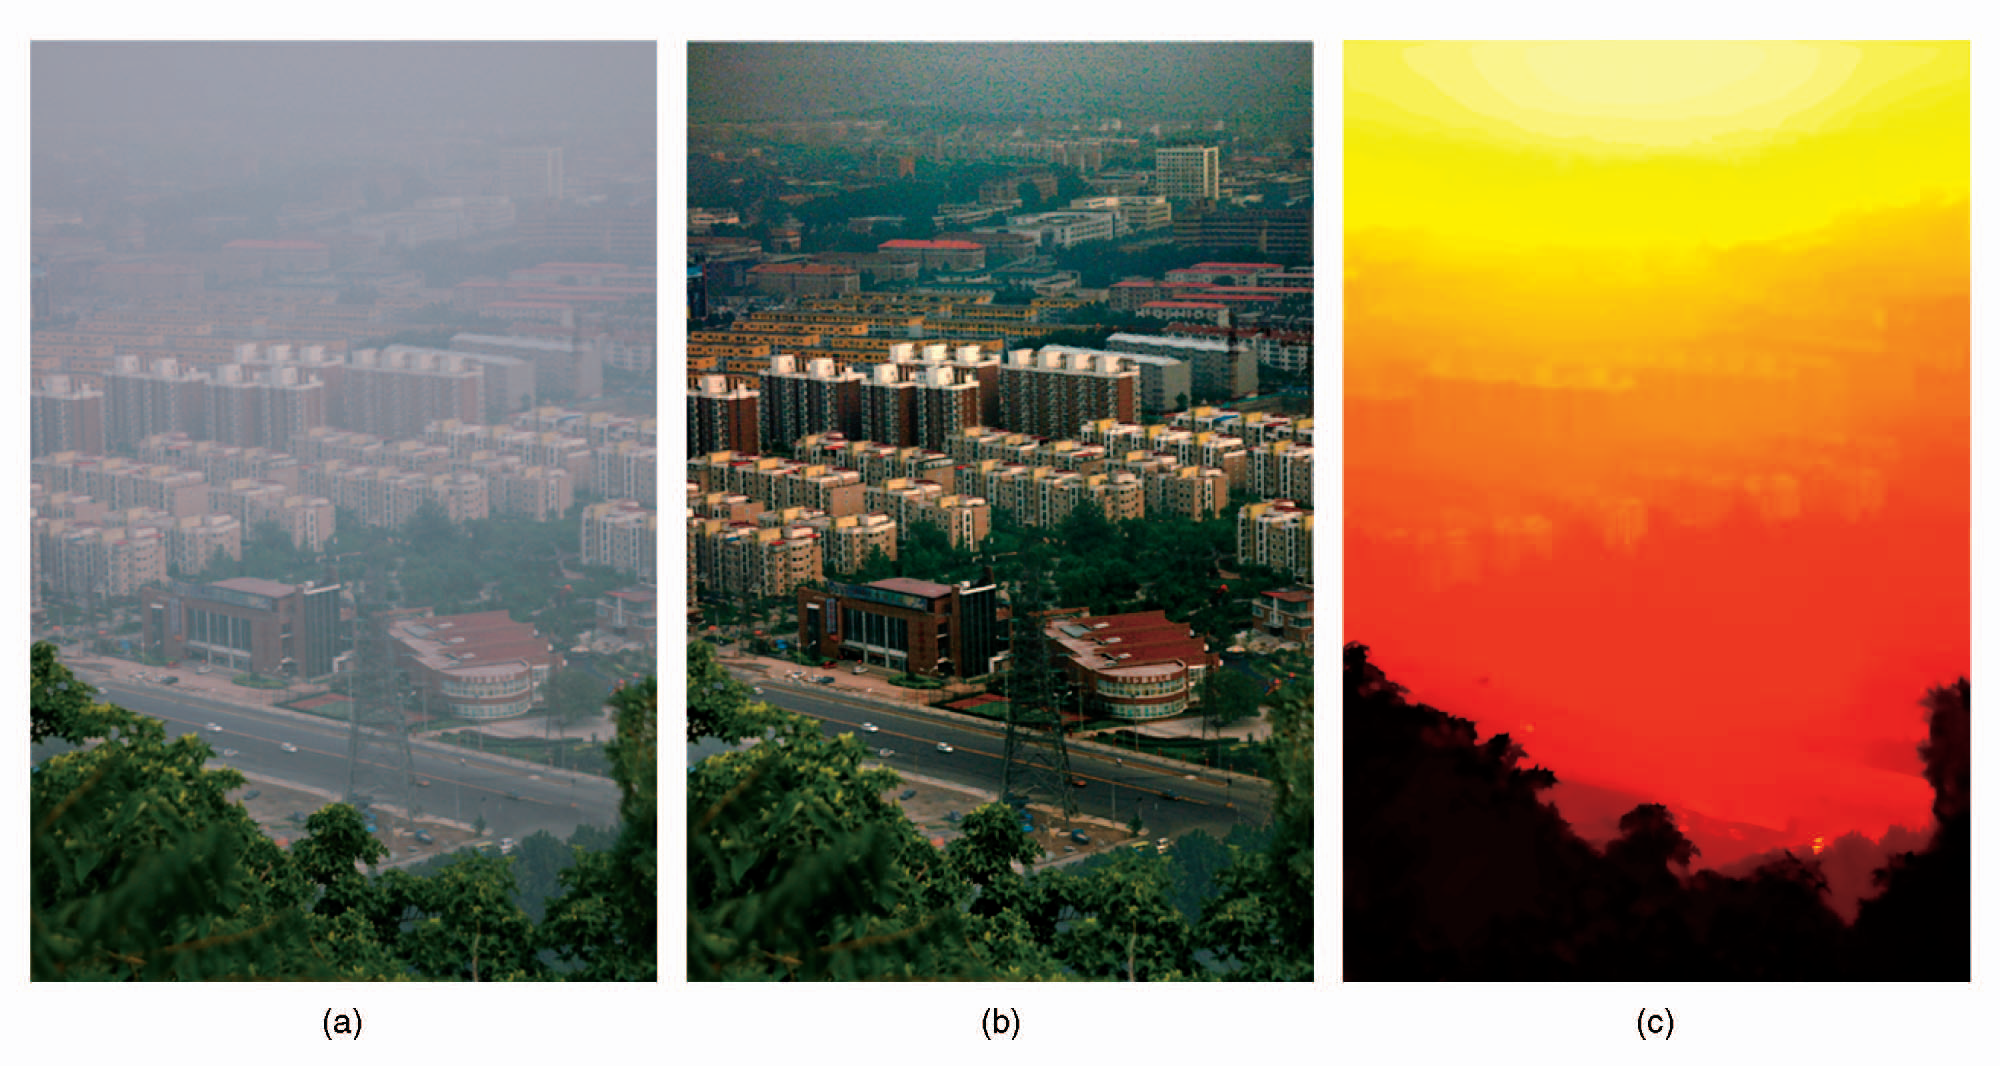
\includegraphics[width=\textwidth]{img/02.png}
    \caption{Haze removal using a single image. (a) Input hazy image. (b) Image after haze removal by our approach. (c) Our recovered depth map.}
    \label{fig:01}
\end{figure}


\section{背景}
在计算机视觉和计算机图形学中,下述模型\cite{NarasimhanNayar2002},\cite{NarasimhanNayar2000},\cite{Fattal2008},\cite{Tan2008},广泛用于描述有雾图像的形成:

\begin{equation}\label{equ:1}
    I(x) = J(x)t(x) + A(1 - t(x)),
\end{equation}

其中$I$是指观测强度,$J$是景物光线强度,$A$是全球大气光,$t$是介质透射率,用来描述到照相机过程中没有被散射的部分光线。去雾的目标就是从$I$中复原$J$,$A$,$t$。对于一个有\emph{N}个像素的彩色图像$I$来说,存在3\emph{N}的已知项和$4\emph{N}+3$的未知项。这就使得雾霾的去除问题变得模糊不清。\par

在\ref{equ:1}中,右边第一项$J(x)t(x)$叫做\emph{直接衰减项}\cite{Tan2008},第二项$A(1 - t(x))$叫做\emph{大气光}\cite{Koschmieder1924},\cite{Tan2008}。直接衰减项描述景物光线,并在介质中衰减,大气光来源于先前散射的光线,并导致色偏。直接衰减项是景物光线的\emph{乘性}失真时,大气光则是\emph{加性}失真。\par

当大气光均匀时,透射率$t$可表达为:

\begin{equation}\label{equ:2}
    t(x) = e^{-\beta d(x)},
\end{equation}

其中$\beta$是大气的散射系数,$d$是场景深度。该式表明景物光线是随着景深按指数衰减的。如果我们可以恢复出透射率,我们就可以恢复出未知范围内的景深。\par

从几何学来看,雾图方程\ref{equ:1}意味着,在RGB色彩空间中,向量$A$,$J(x)$,$I(x)$是共面的,它们的端点则是共线的,透射系数$t$是两条线段长度之比:

\begin{equation}\label{equ:3}
    t(x) = \frac{\| A - I(x) \|}{\| A - J(x) \|} = \frac{A^c - I^c(x)}{A^c - J^c(x)},
\end{equation}

其中$c \in \{r, g, b\} $为颜色通道索引。\par

\begin{figure}[bp]
    \centering
    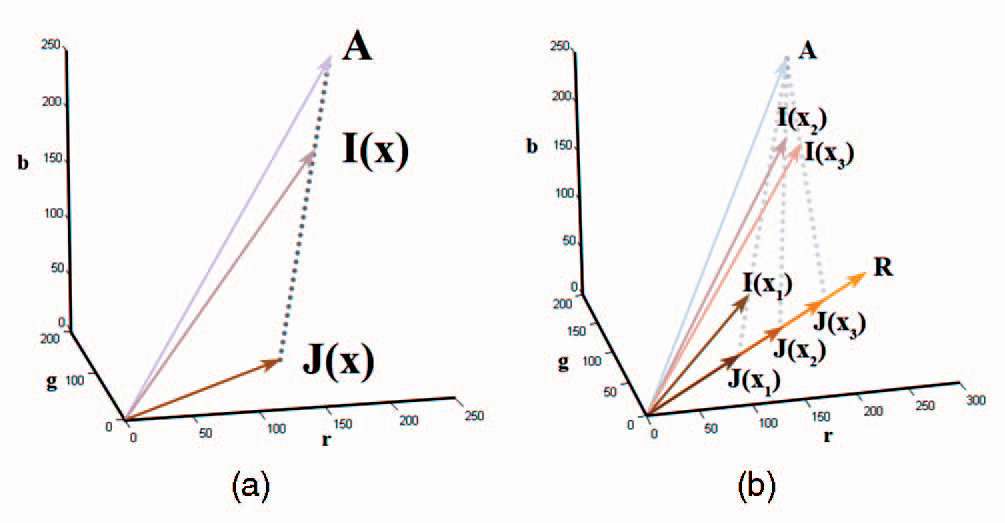
\includegraphics[width=0.5\textwidth]{img/01.png}
    \caption{(a) Haze imaging model. (b) Constant albedo model used in Fattal’s work \cite{Fattal2008}.}
    \label{fig:02}
\end{figure}

基于这个模型,Tan的方法\cite{Tan2008}主要关注增强图像的能见度上。在透射率$t$可近似看作不变的区域内,由于$t<1$,输入图像的能见度(梯度之和)在雾的干扰之下减少:

\begin{equation}\label{equ:4}
    \sum_x \| \nabla I(x) \| = t \sum_x \| \nabla J(x) \| < \sum_x \| \nabla J(x) \|,
\end{equation}

在一个局部区域内,透射率$t$是通过扩大图像可见度并且使对比度满足$J(x)$的强度低于$A$的方法来估计的。一个MRF模型被用来进一步规范该结果。这一尝试将进一步揭开雾成像的一些细节和结构上的奥秘。然而,这一方法会产生更大的饱和值,因为它只关注可见度的增强而并没有从物理上去复原原始景物的光线。此外,在靠近深度不连续的位置可能会包含一些光环效应。\par

在\cite{Fattal2008}中,Fattal提出了一种基于独立成分分析(ICA)的方法。首先,局部区域的反照率被假定为一个恒定的向量$R$。因而,在该区域内所有的$J(x)$拥有相同的方向向量$R$,如图\ref{fig:02}b所示。其次,通过假定在一个局部表面投影$\|J(x)\|$和透射率函数$t(x)$在统计学上是相互独立的,可以用ICA来估算$R$。最后,由输入的彩色图像建立的MRF模型可用来推断整幅图像的结果。这一实现手段是基于物理的并能产生自然的无雾图像和一幅优质的深度图。不足的是,该手段因为利用了一个局部区域的统计学独立的假设,需要在相互独立的成分之间差异很大的时候才能有显著效果。任意差异性的缺乏或者过低的信噪比(通常出现在浓雾图)都会使得统计结果不可靠。还有,统计规律是根据图像的颜色信息得出的,因此对灰度图像无效。面对无色的浓度较大雾时,该方法也无能为力。\par

在下一章,我们将展示一种新的先验规律——暗通道先验,并用来直接评估户外有雾图像的透射率。\par

\section{暗通道先验}
暗通道先验是通过对户外无雾图像的观察得出的:在绝大多数非天空的局部区域里,某一些像素总会有至少一个颜色通道具有很低而且接近于零的值。换言之,该区域光强度的最小值是个接近零的数。\par

为了用公式描述这个发现,对于一幅图像$J$,我们定义\emph{暗通道}的概念。对于特定图像$J$,它的暗通道$J^{dark}$取决于

\begin{equation}\label{equ:5}
    J^{dark}(x) = \min_{y \in \Omega(x)}\Big(\min_{c \in \{ r, g, b\}} J^c(x)\Big),
\end{equation}

其中$J^c$代表$J$的某一个颜色通道,而$\Omega(x)$是以$x$为中心的一块方形区域。暗通道由两个求最小值操作得出:$\min_{c \in \{ r, g, b\}}$对应每个像素(图\ref{fig:03}b),$\min_{y \in \Omega(x)}$是一个最小值过滤器(MinFilter,图\ref{fig:03}c)。两个求最小值操作可交换。\par

\begin{figure}[tbp]
    \centering
    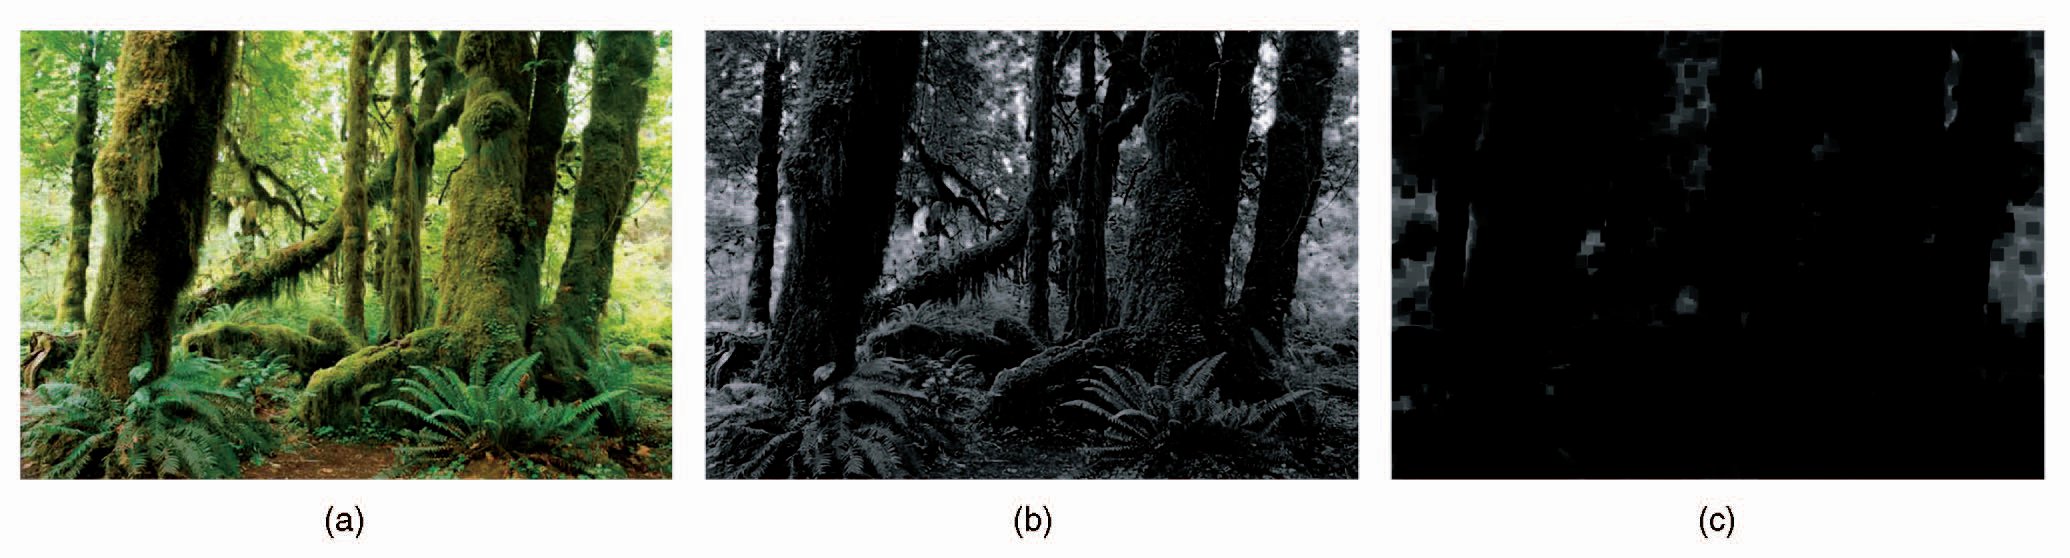
\includegraphics[width=\textwidth]{img/03.png}
    \caption{Calculation of a dark channel. (a) An arbitrary image $J$. (b) For each pixel, we calculate the minimum of its (r, g, b) values. (c) A minimum filter is performed on (b). This is the dark channel of $J$. The image size is 800 $\times$ 551, and the patch size of $\Omega$ is 15 $\times$ 15.}
    \label{fig:03}
\end{figure}

使用暗通道的概念,我们观察得出,如果$J$是户外的无雾图像,除了天空方位,$J$的暗通道强度总是很低并且趋近于零。

\begin{equation}\label{equ:6}
    J^{dark} \to 0
\end{equation}

我们把这一发现称为\emph{暗通道先验}。\par

造成暗通道的低强度值的因素主要有三个:a)阴影,比如汽车、建筑物和城市中玻璃窗户的阴影,或者是树叶、树与岩石等自然景观的投影;b)色彩鲜艳的物体或表面,比如在任何通道中的反射值都很低(比如绿色的草地、树、植物,红色或黄色的花朵、叶子,或者蓝色的水面);c)颜色较暗的物体或者表面,例如灰暗色的树干和石头。总之,自然的户外景物中到处都是阴影或者彩色,这些景物的图像的暗通道总是很灰暗的!\par

为了验证暗原色先验的表现有多好,我们从Flickr.com 和其他一些图片搜索引擎上使用Flickr用户标记的150个最热门的标签,收集了一个户外图像的数据库,因为雾主要出现在户外景物或者城市中,我们从下载到的图像中主要选出了这两部分景区的无雾图像。另外,我们只研究了白天的图像。我们随机选取了5,000张图像并手工去掉了包括天空区域的部分。它们均被缩放成最大长宽都是500像素的大小,用$15 \times 15$的步长计算出暗通道。图\ref{fig:04}显示了几幅户外图像以及相应的暗通道。\par

\begin{figure}[tbp]
    \centering
    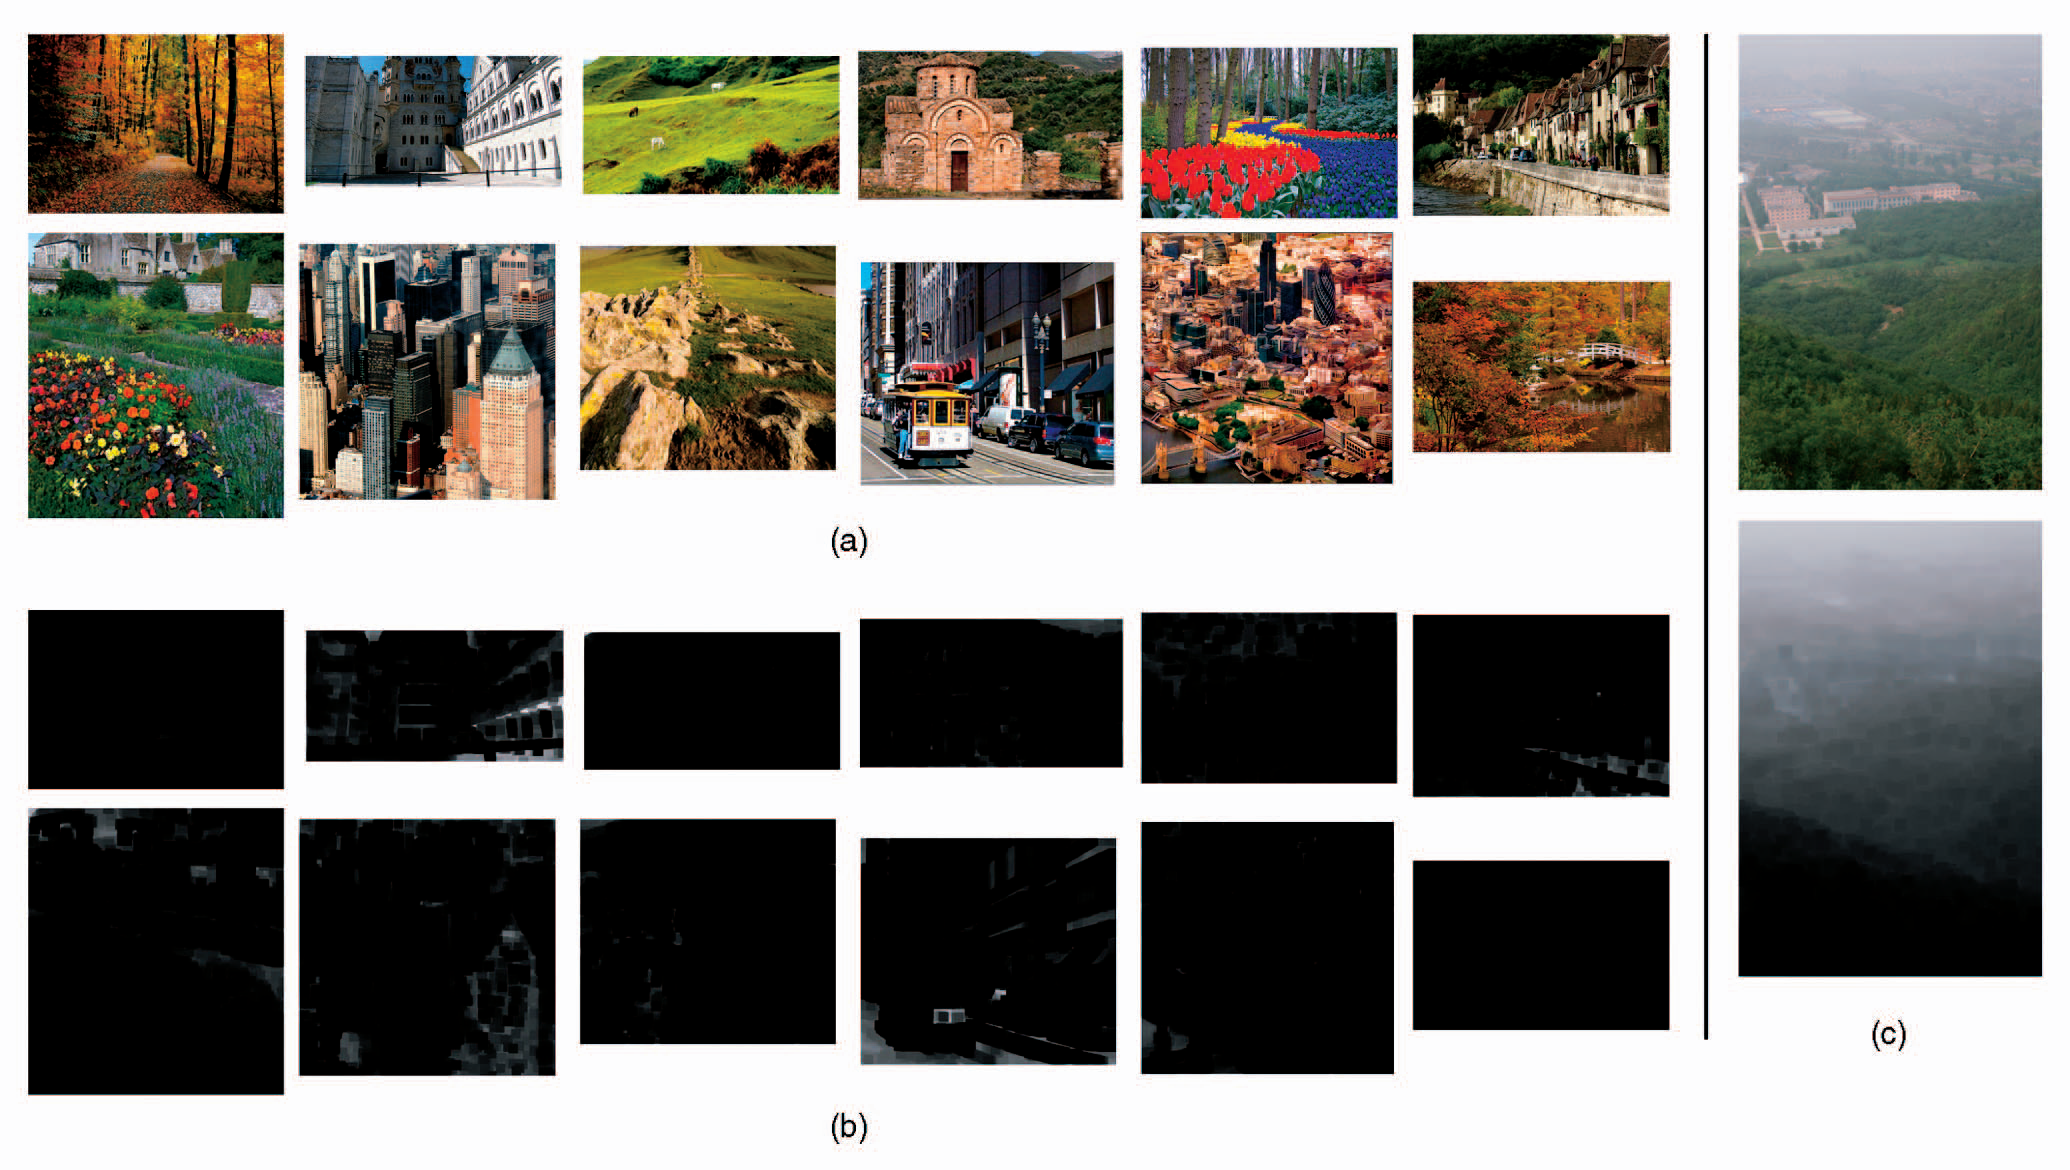
\includegraphics[width=\textwidth]{img/04.png}
    \caption{(a) Example images in our haze-free image database. (b) The corresponding dark channels. (c) A hazy image and its dark channel.}
    \label{fig:04}
\end{figure}

\begin{figure}[bp]
    \centering
    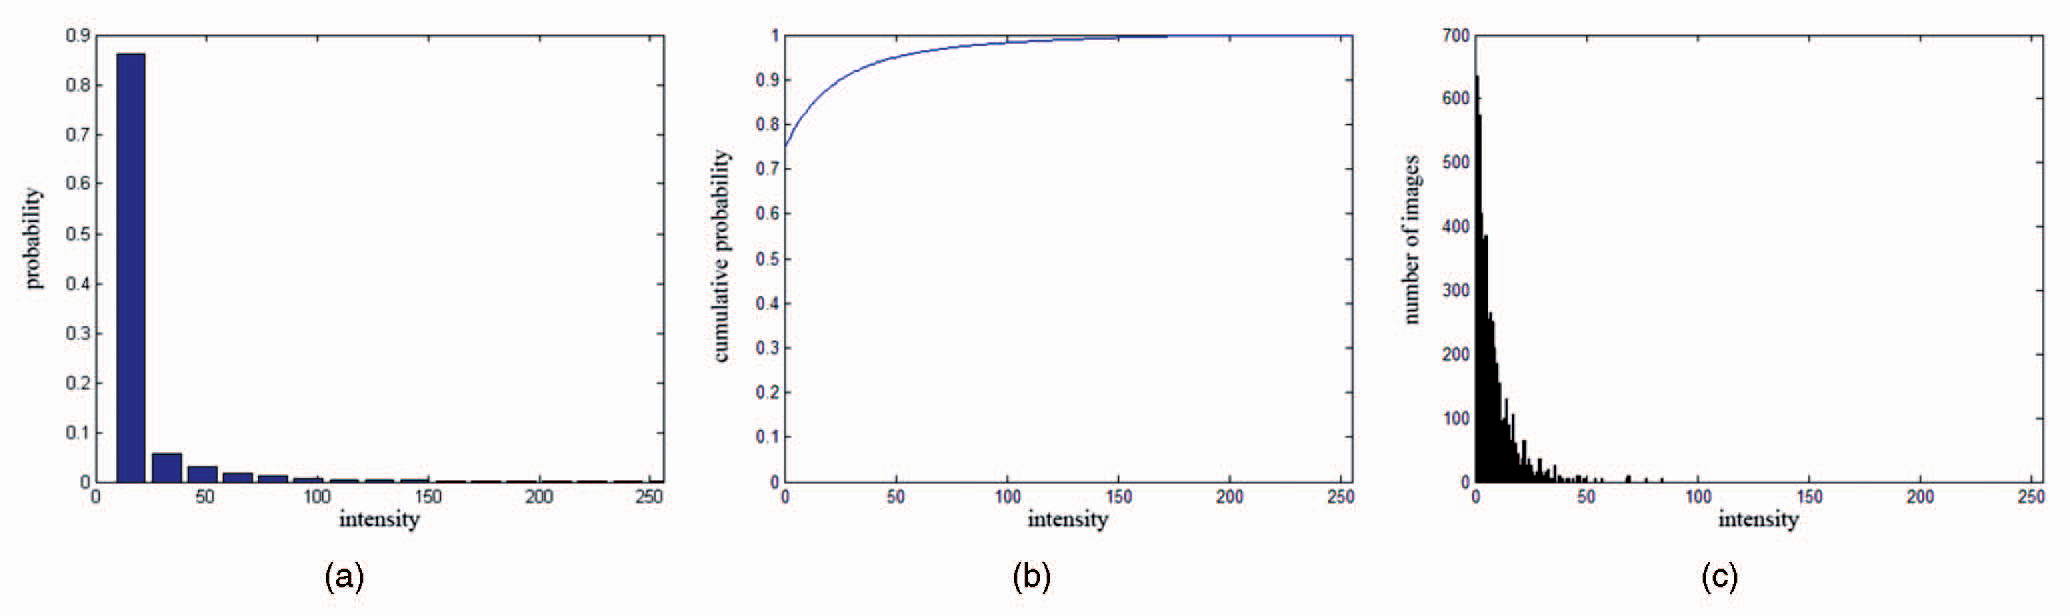
\includegraphics[width=\textwidth]{img/05.png}
    \caption{Statistics of the dark channels. (a) Histogram of the intensity of the pixels in all of the 5,000 dark channels (each bin stands for 16 intensity levels). (b) Cumulative distribution. (c) Histogram of the average intensity of each dark channel.}
    \label{fig:05}
\end{figure}

图\ref{fig:05}a是超过5,000幅图像的暗通道强度直方图,图\ref{fig:05}b是相应的累计直方图。我们可以看到暗通道当中约有75\%的像素强度值为零,大概90\%的像素强度值低于25。该统计结果强有力地支持了暗通道先验的合理性。我们同时还计算了每幅图像暗通道像素的平均强度值,其直方图如图\ref{fig:05}所示。同样,大多的暗通道都具有比较低的平均强度值。这就意味着只有极少数的户外无雾图像不符合我们的先验规律。\par

由于附加的大气光,图像被雾干扰之后往往要比其本身亮度更大,透射率$t$一般较小。所以被浓雾覆盖的图像的暗通道具有较高的强度值(见图\ref{fig:04}右手边)。视觉上来看,暗通道强度值是雾浓度的粗略近似。在下一部分,我们将利用这一性质来估算透射和大气光。\par

可以看到,我们忽视了天空区域,因为该处无雾图像的暗通道具有较高的强度值。幸好,可以利用雾图生成模型\ref{equ:1}结合我们所提出的先验优雅地处理天空区域。没有必要特意去除天空区域,我们将在\ref{sec:4.1}章讨论这个问题。\par

我们的暗通道先验的一定程度上受到了众所周知的广泛用于多光谱传感系统的黑体减法(dark-object subtraction)技术\cite{Chavez1988}的启发。在\cite{Chavez1988}中,通过减去场景中最暗物体所对应的一个常数来去除空间各向同性的雾。我们从这个想法中归纳得到了新的自然风景图去雾的途径。\par



\section{使用暗通道先验去雾}

    \subsection{估算透射率}\label{sec:4.1}
    我们首先假设大气光$A$是给定的,在\ref{sec:4.3}章我们会展示一种自动评估大气光的途径。我们先用$A$正则化雾图生成方程\ref{equ:1}:

    \begin{equation}\label{equ:7}
        \frac{I^c(x)}{A^c} = t(x)\frac{J^c(x)}{A^c}  + 1 - t(x),
    \end{equation}

    注意到我们对每个颜色通道分别做正则化。\par

    \subsection{软抠图(Soft Matting)} %这里还是不翻译比较好

    \subsection{估算大气光}\label{sec:4.3}

    \subsection{复原场景光线}

    \subsection{窗口大小}


\section{实验结果}

\section{讨论}


\bibliographystyle{unsrt}
\bibliography{refs}
\end{document}